%!TEX root=ClockPendulumAnalyzer.tex
\section{Raspberry Pi}
\begin{frame}
%image with all the technologies
\end{frame}

\subsection{Aufbau - Architektur}
\begin{frame}
    \frametitle{Aufbau - Architektur}
    \begin{columns}[c] % the "c" option specifies center vertical alignment
        \column{.5\textwidth}
        \begin{itemize}
            \item<1->3-Layer Architektur
            \item<1->mögliche 2-Tier Verteilung
            \item<1->Daten-Transfer-Objekt und REST
        \end{itemize}
        \column{.5\textwidth} % column designated by a command
        \begin{figure}
            \centering
            \begin{overprint}
                \onslide<1>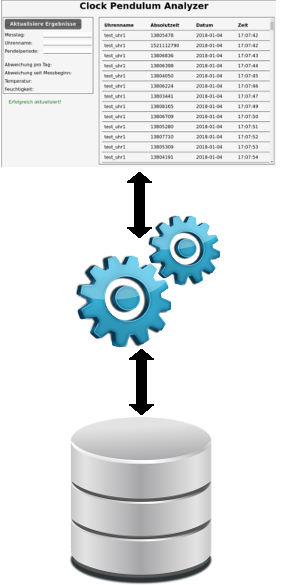
\includegraphics[width=.5\textwidth]{3layer.png}
                \onslide<2->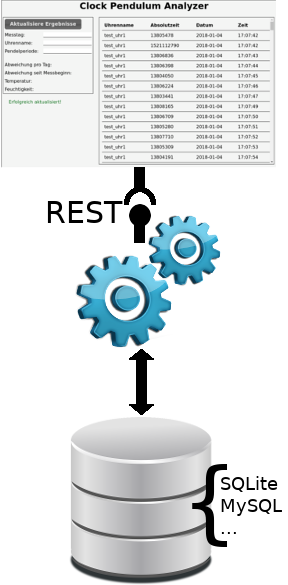
\includegraphics[width=.5\textwidth]{3layer_rest.png}
            \end{overprint}
        \end{figure}
    \end{columns}
\end{frame}

\subsection{C++ Software}
\begin{frame}
    \frametitle{C++ Software Feature}
    \begin{columns}[c] % the "c" option specifies center vertical alignment
        \column{.5\textwidth}
        \begin{itemize}
            \item<1-> Observer Pattern $\rightarrow$ UARTReceiver
            \item<1-> Interface Segregation und Interface Abstraktion
            \item<1-> Ressource acquisition is initialization
            \item<1-> Multithreading von UART, REST und Main
        \end{itemize}
        \column{.5\textwidth} % column designated by a command
        \begin{figure}
            \centering
            \begin{overprint}
                \onslide<1>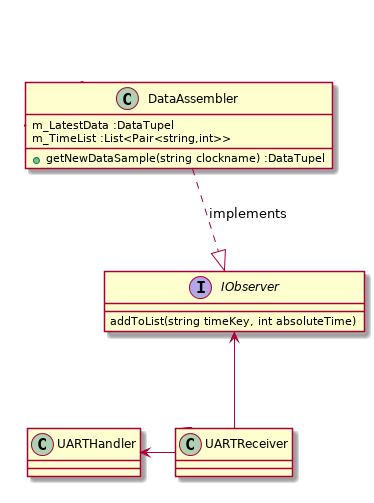
\includegraphics[width=.8\textwidth]{cppfeature_observer.png}
                \onslide<2>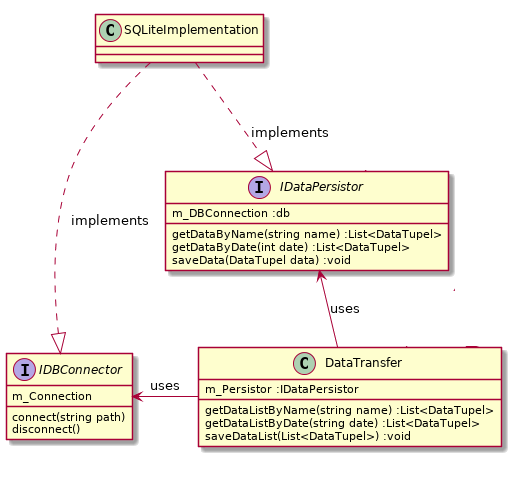
\includegraphics[width=.8\textwidth]{cppfeature_isp.png}
                \onslide<3>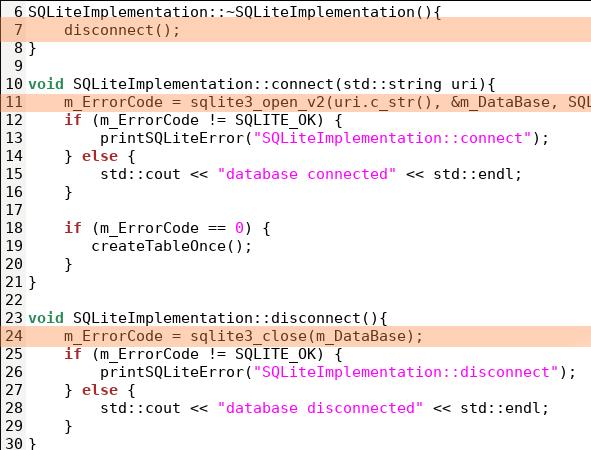
\includegraphics[width=\textwidth]{raii.png}
            \end{overprint}
        \end{figure}
       
    \end{columns}
\end{frame}

\subsection{REST Service}
\begin{frame}
    \frametitle{REST Service}
    \begin{itemize}
        \item Einfacher Aufruf auf Daten von ausserhalb
        \begin{itemize}
            \item Uhrenname, Datum, Zeit, Absolute Ticks und Referenz
            \item \textit{192.168.192.75:8080/?name=test\_uhr1\&date=20180104\%}
        \end{itemize}
        \item TCP Socket auf Port 8080
        \item Abkopplung des Zugriffs
    \end{itemize}
\end{frame}

\subsection{Web Oberfläche}
\begin{frame}
    \frametitle{Web Oberfläche}
    \begin{itemize}
        \item primitive Benutzeroberfläche
        \item basiert auf einfachem Javascript und HTML
        \item unabhängige eigene Applikation $\rightarrow$ 2-Tier Architektur
    \end{itemize}
    \begin{figure}
        \centering
        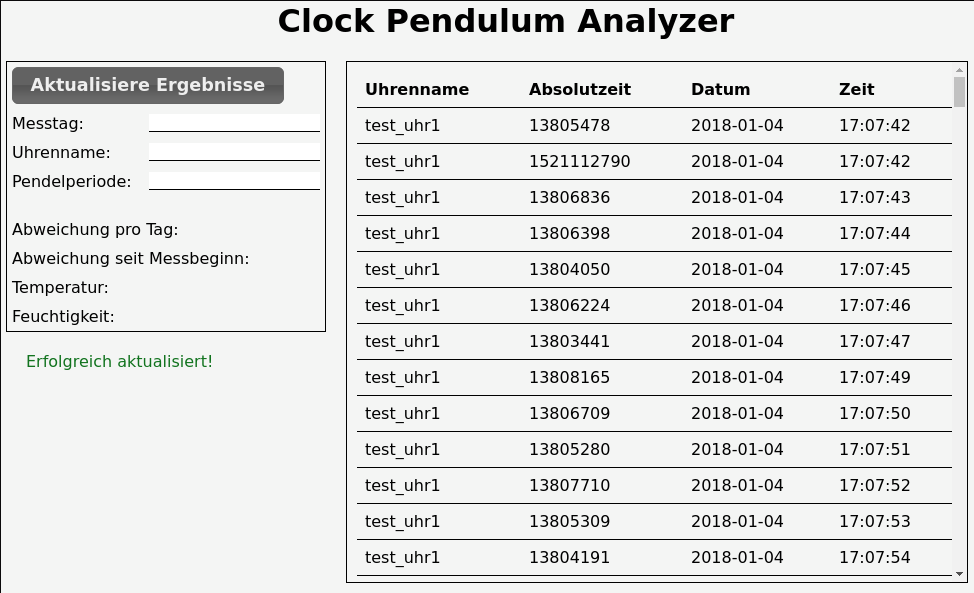
\includegraphics[width=.7\textwidth]{browser.png}
    \end{figure}
\end{frame}

\subsection{Demo}
\begin{frame}
\centering
{\LARGE Live - Demo}
\vspace{1.5cm}

\color{blue}\url{http://192.168.192.75/}
\end{frame}